\documentclass[border=10pt]{standalone}

\usepackage{tikz}
\usepackage{tikzsymbols}
\usetikzlibrary{calc,patterns,shapes.geometric}

\def\centerarc[#1](#2)(#3:#4:#5){\draw[#1] ($(#2)+({#5*cos(#3)},{#5*sin(#3)})$) arc (#3:#4:#5);}

\begin{document}
	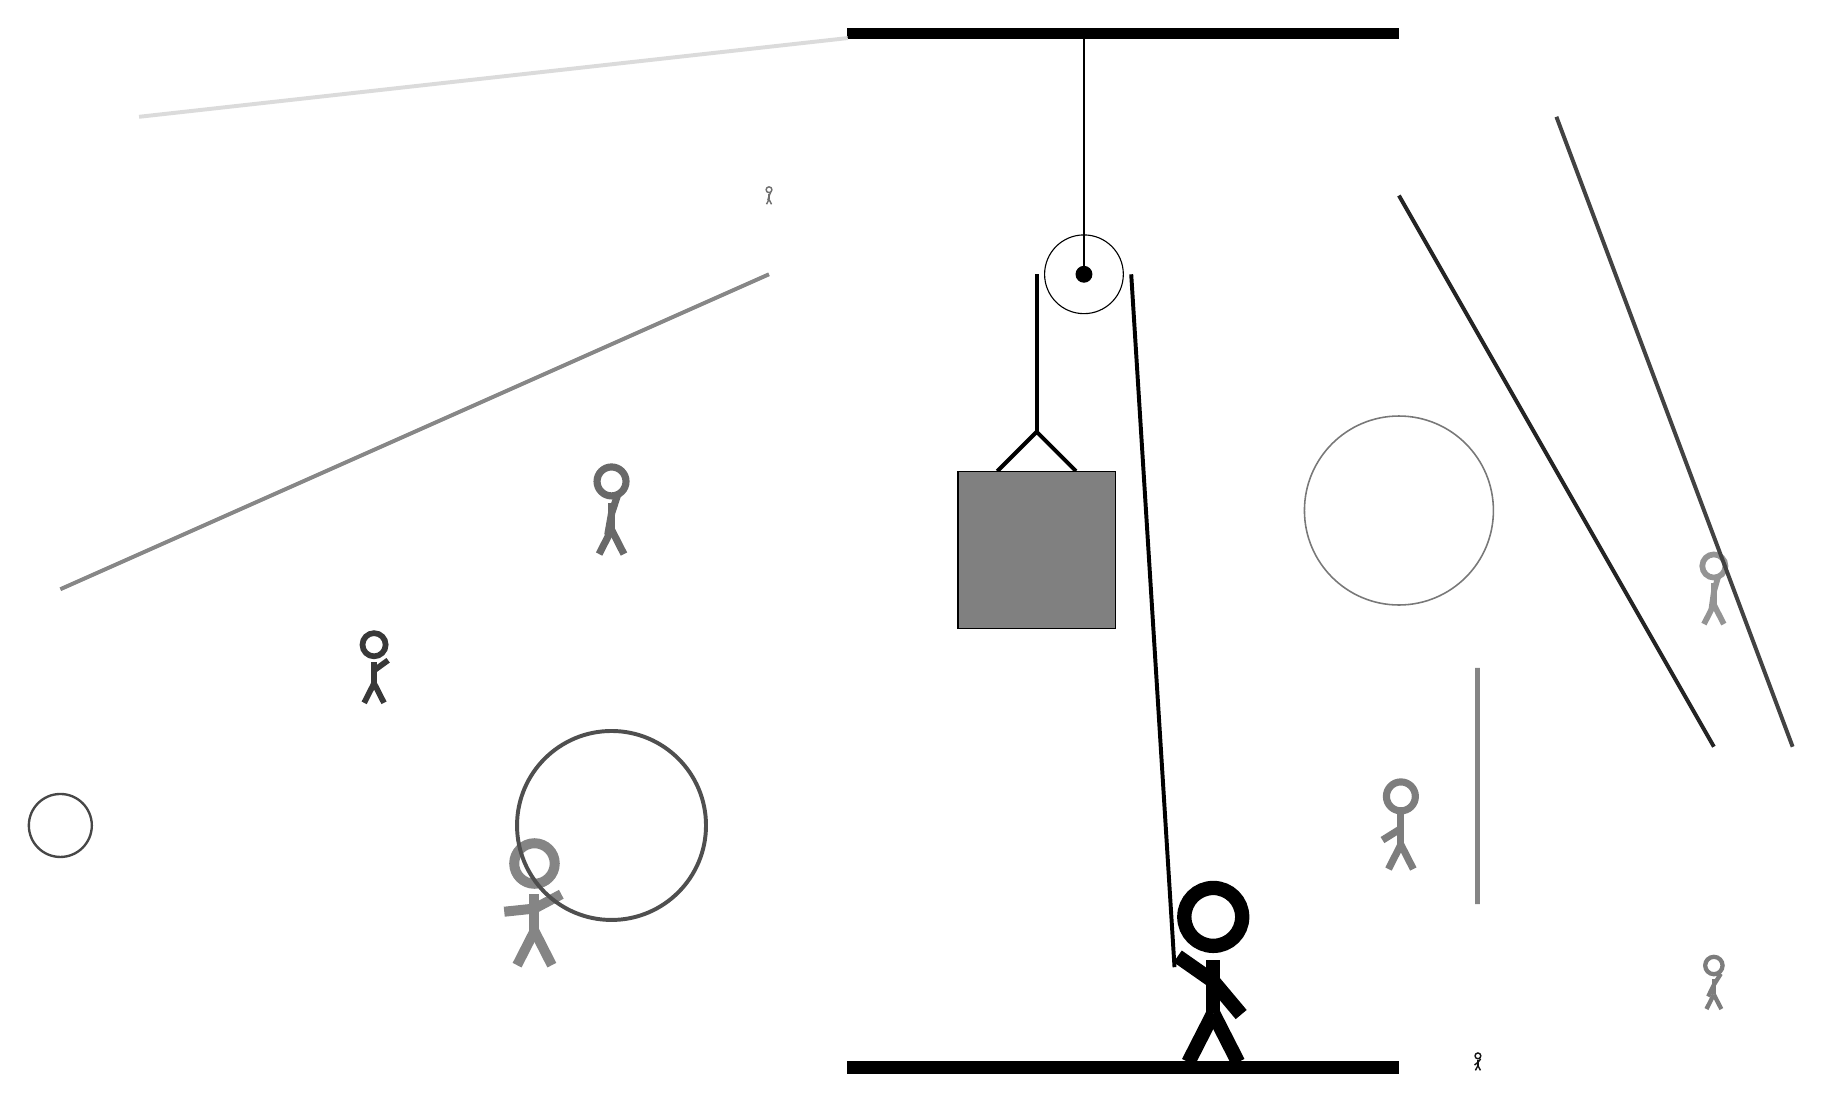
\begin{tikzpicture}
		%%%%% START %%%%%
		
		\draw[fill=black] (-2, 10) rectangle (5, 10.125);
		
		\draw (1, 7) circle (0.5);
		\draw[fill=black] (1, 7) circle (0.1);
		\draw (1, 10) -- (1, 7);
		
		\draw[line width=0.5mm] (-0.1, 4.5) -- (0.4, 5.0) -- (0.9, 4.5);
		\draw[fill=black!50] (-0.6, 4.5) rectangle (1.4, 2.5);
		
		\draw[line width=0.5mm] (0.4, 7) -- (0.4, 5.0);
		\centerarc[line width=0.5mm](1, 7)(0:180:0.6);
		\draw[line width=0.5mm](1.6, 7) -- (2.15, -1.8);
		
		\node at (2.6, -1.9) {\Strichmaxerl[10][-35][-50]};
		
		\draw[line width=0.5mm, color=black!47](-3, 7) -- (-12, 3);
		
		\node[line width=0.4mm, color=black!59] at (-5, 4) {\Strichmaxerl[5][80][72]};
		\node[line width=0.2mm, color=black!51] at (9, -2) {\Strichmaxerl[3][64][58]};
		\node[line width=0.7mm, color=black!57] at (-3, 8) {\Strichmaxerl[1][74][67]};
		\node[line width=0.6mm, color=black!78] at (-8, 2) {\Strichmaxerl[4][89][36]};
		\node[line width=0.7mm, color=black!48] at (-6, -1) {\Strichmaxerl[7][6][28]};
		\node[line width=0.3mm, color=black!42] at (9, 3) {\Strichmaxerl[4][82][74]};
		\draw[line width=0.5mm, color=black!74](10, 1) -- (7, 9);
		\draw [line width=0.2mm, color=black!53](5, 4) circle (1.2);
		\draw [line width=0.5mm, color=black!69](-5, 0) circle (1.2);
		\draw[line width=0.6mm, color=black!48] (6, 2) rectangle (6, -1);
		\draw [line width=0.3mm, color=black!72](-12, 0) circle (0.4);
		\node[line width=0.7mm, color=black!51] at (5, 0) {\Strichmaxerl[5][32][90]};
		
		\draw[line width=0.5mm, color=black!14](-2, 10) -- (-11, 9);
		\node[line width=0.2mm, color=black!92] at (6, -3) {\Strichmaxerl[1][38][51]};
		\draw[line width=0.5mm, color=black!86](9, 1) -- (5, 8);
		
		
		\draw[fill=black] (-2, -3) rectangle (5, -3.15);
		
		%%%%% END %%%%%
	\end{tikzpicture}
\end{document}